\documentclass[12pt, a0paper, portrait, margin=0mm, innermargin=0mm]{tikzposter}
\geometry{paperwidth=36in, paperheight=20.25in, margin=0in}
\usepackage{adjustbox}
\usepackage{amsmath}
\usepackage{booktabs}
\usepackage{enumitem}
\usepackage[T1]{fontenc}
\usepackage{graphicx}
\usepackage[font=large, labelfont=bf]{caption}
\usepackage{capt-of}
\usepackage{helvet}
\usepackage{hyperref}
\usepackage[capitalise]{cleveref}
\usepackage{multicol}
\usepackage{nth}
\usepackage{siunitx}
\usepackage{wrapfig}
\usepackage{xcolor}

\definecolor{um-maize}{cmyk}{0, 0.18, 1, 0}
\definecolor{um-blue}{cmyk}{1, 0.60, 0, 0.60}

\usetheme{Board}

\useblockstyle{Slide}
\defineblockstyle{sampleblockstyle}{
	titlewidthscale=0.9, bodywidthscale=1,titleleft,
	titleoffsetx=0pt, titleoffsety=0pt, bodyoffsetx=0mm, bodyoffsety=5mm,
	bodyverticalshift=10mm, roundedcorners=5, linewidth=2pt,
	titleinnersep=2mm, bodyinnersep=1cm
}{
	\draw[color=framecolor, fill=blockbodybgcolor,
	rounded corners=\blockroundedcorners] (blockbody.south west)
	rectangle (blockbody.north east);
	\ifBlockHasTitle
	\draw[color=framecolor, fill=blocktitlebgcolor,
	rounded corners=\blockroundedcorners] (blocktitle.south west)
	rectangle (blocktitle.north east);
	\fi
}

% COLOR
\colorlet{backgroundcolor}{white}
\colorlet{blocktitlebgcolor}{um-maize}
\colorlet{blocktitlefgcolor}{um-blue}

\tikzposterlatexaffectionproofoff

\title{0.55T Prostate Diffusion-Weighted Imaging Using Multi-Shot EPI and Self-Supervised Learning Reconstruction}
\author{Zhengguo Tan ({\color{um-blue}zgtan@umich.edu}), Jacob Richardson, Thomas L Chenevert, Hero Hussain, Michael Jaroszewicz, Yun Jiang, Nicole Seiberlich, Vikas Gulani}
\institute{Department of Radiology, University of Michigan, Ann Arbor, MI, USA}

\newcommand{\argmin}{\operatornamewithlimits{argmin}}
\newcommand{\norm}[1]{\left\lVert#1\right\rVert}

% BLOCK HEIGHT
\newlength\htblockbox
\newcommand{\mtblock}[3]{%
	\block{#2}{%
		\setlength{\htblockbox}{#1}%
		\parbox[t][\htblockbox][c]{\linewidth}{#3}}}


\begin{document}
	
	\maketitle
	
	\node[anchor=west] at (TP@title.west) {\includegraphics[width=8cm]{figures/um.png}};
	
	\begin{columns}
		\column{0.33}
		\mtblock{5cm}{1. INTRODUCTION}{
			About 1 in 8 American men will develop prostate cancer in their lifetime, 
			with risk increasing significantly with age. 
			$T_2$-weighted imaging and diffusion-weighted imaging (DWI) are identified by PI-RADS [1]
			as key image contrasts for noninvasive diagnosis and assessment of prostate cancer.
			At field strength widely adopted in clinical practice (1.5T and above), however, 
			DWI suffers from degraded and undiagnosable images for patients with hip imaplants 
			due to its strong magnetic field inhomogeneity. 
			Recently, 0.55T shows special values for patients with large habitus or metallic implants 
			given its reduced field inhomogeneity. 
			The major challenge at 0.55T is its reduced signal-to-noise ratio (SNR).
			Therefore, this study aims to \textbf{leverage accelerated multi-shot EPI and 
			self-supervised reconstruction unrolling ADMM (alternating direction method of multipliers)
			to boost the resolution and SNR of DWI and to enable high-quality prostate imaging at 0.55T}.
		}
		
		\mtblock{25cm}{2.1. METHOD - Multi-Shot EPI: Boost Resolution}{
			
			\begin{wrapfigure}{r}{0.63\linewidth}
				\centering
				\includegraphics[width=\linewidth]{figures/sampling.png}
				\caption{Undersampled 2-shot EPI acquisition with shifted encoding.}
				\label{FIG:SAMPLING}
			\end{wrapfigure}

			The first two sub-figures in Figure \ref{FIG:SAMPLING} displays 
			the employed 2-shot interleaved EPI acquisition with 4-fold acceleration per shot.
			The last sub-figure depicts the shifted encoding scheme. 
			Here, every two columns represent the acquisition of one diffusion direction 
			(as shown with the same color), 
			and the acquired phase-encoding lines in one direction are shifted by one line 
			with respect to the preceding direction,
			achieving complementary $k$-$q$-space sampling [2].
			
			\setlength{\parindent}{2em} For prostate DWI, 
			the 3-scan trace diffusion mode was employed in both acquisition protocols (Table \ref{TAB}).
			After image reconstruction, trace-weighted images were computed as 
			geometric means of all diffusion-weighted images with the same $b$-value.
			Subsequently, the apparent diffusion coefficient (ADC) map can be fitted from:
			\begin{equation}
				\mathrm{TRACE}_i = b_0 \cdot e^{-b_i \cdot \mathrm{ADC}}.
			\end{equation}
			$i$ denotes the index of different $b$-values and 
			$b_0$ denotes the non-diffusion-weighted spin-echo image.
			
			\newcolumntype{a}{p{0.30\linewidth}}
			\newcolumntype{b}{p{0.08\linewidth}}
			\begin{wrapfigure}{r}{0.70\linewidth}
				\captionof{table}{Acquisition protocols.}
				\begin{center}
					\begin{tabular}{a | b b b | b b b}
						\toprule
						\textbf{Protocol} & \multicolumn{3}{c|}{\textbf{\#1 ($3.5\times2.3$~mm$^2$)}} & \multicolumn{3}{c}{\textbf{\#2 ($1.6\times1.6$~mm$^2$)}} \\
						\hline
						FOV (mm) & \multicolumn{6}{c}{240} \\
						slice thickness (mm) & \multicolumn{6}{c}{4} \\
						slices & \multicolumn{6}{c}{15} \\
%						diffusion mode & \multicolumn{6}{c}{3-scan trace} \\
						$b$-values (\si{s/mm2}) & 50, & 500, & 800 & 50, & 500, & 800 \\
						averages & 3, & 12, & 27 & 1, & 12, & 16 \\
						magnetization prep. & \multicolumn{3}{c|}{slice-sel.~IR (145~ms)} & \multicolumn{3}{c}{fat sat}\\
						base resolution & \multicolumn{3}{c|}{106} & \multicolumn{3}{c}{150} \\
						phase resolution (\%) & \multicolumn{3}{c|}{65} & \multicolumn{3}{c}{100} \\
						shots & \multicolumn{3}{c|}{1} & \multicolumn{3}{c}{2} \\
						acceleration & \multicolumn{3}{c|}{3} & \multicolumn{3}{c}{2} \\
						partial Fourier & \multicolumn{3}{c|}{7/8} & \multicolumn{3}{c}{5/8} \\
						TE/TR (ms) & \multicolumn{3}{c|}{74/3630} & \multicolumn{3}{c}{83/2800} \\
						acquisition (\si{\minute}) & \multicolumn{3}{c|}{8:26} & \multicolumn{3}{c}{8:15} \\
						\bottomrule
					\end{tabular}\label{TAB}
				\end{center}
			\end{wrapfigure}
			
			\cref{TAB} lists key acquisition parameters of the single-shot (\#1) and the two-shot (\#2) protocol,
			respectively. Protocol \#2 with the use of accelerated 2-shot acquisition boosts spatial resolution 
			without elongated echo spacing and echo train length. 
			In addition, we employed fewer averages than Protocol \#1 to match the scan time for both protocols.
			
			Scans at \SI{0.55}{\tesla} (Free.Max, Siemens Healthineers, Erlangen, Germany) with contour coils 
			were conducted on the diffusion phantom (CaliberMRI, Boulder, CO, USA) and 
			five male subjects with written consent in compliance with IRB.
		}
		
		\column{0.33}
		\mtblock{19cm}{2.2. METHOD - Self-Supervised ADMM Unrolling: Boost SNR}{
			
			\begin{wrapfigure}{r}{0.50\linewidth}
				\centering
				\includegraphics[width=\linewidth]{figures/unroll.png}
				\caption{ADMM unrolling for multi-shot EPI.}
				\label{FIG:UNROLL}
			\end{wrapfigure}
			
			We extended the self-gated self-supervised ADMM unrolled reconstruction [3,4] 
			for prostate DWI at \SI{0.55}{\tesla}, 
			formulating a joint $k$-$q$-space minimization problem:
			
			\begin{equation}
				\argmin_x \norm{ y - \mathcal{A} x }_2^2 + \lambda \cdot \mathcal{R} x
				\label{EQU:MINFUNC}
			\end{equation}

			$y$ and $x$ denotes the acquired multi-coil multi-shot multi-$b$ $k$-space data, 
			and diffusion-weighted images from all diffusion encodings, respectively. 
			The forward operator $\mathcal{A}$ is composed by a chain of linear operators: 
			$\mathbf{P} \mathbf{F} \mathbf{S} \mathbf{\Phi}$, where the input $x$ is multiplied with 
			shot-to-shot phase variation ($\mathbf{\Phi}$), coil sensitivities ($\mathbf{S}$), 
			Fourier trainsformed ($\mathbf{F}$), and masked by the sampling pattern ($\mathbf{P}$).
			
			\setlength{\parindent}{2em} Figure \ref{FIG:UNROLL} illustrates 
			the proposed self-supervised ADMM unrolling. 
			\textbf{(A)} the $k$-space sampling pattern is split into three disjoint sets: 
			the training mask ($\mathbf{T}$) used for the data consistency term in Equation \ref{EQU:MINFUNC},
			and the training ($\mathbf{T}$) and validation ($\mathbf{L}$) masks for the loss function 
			as proposed in SSDU [5], respectively.
			\textbf{(B,C)} depicts the use of these masks during training and validation. 
			$\mathcal{D}_\omega$ denotes the 2D ResNet parameterized by $\omega$ [6], 
			used as the learnable regularization function $\mathcal{R}$.
			\textbf{(D)} This work employed the 2D spatial-diffusion convolution within ResNet, 
			where the diffusion-encoding dimension was stacked in the channel dimension in 'conv2d'.
			Therefore, convolution kernels loop through all diffusion-weighted contrast to learn
			the key features of the high-dimensional data and to reduce noisy and aliasing artifacts 
			in unrolled reconstruction.
			
			Given the anatomical complexisy of prostate, each slice was trained and tested separately. 
%			The training of a generalized model in the self-supervised manner is yet to be explored. 
			All reconstructions were done on A40 GPU with \SI{40}{\giga\byte} memory 
			(NVIDIA, Santa Clara, CA, USA) from the Great Lakes HPC Cluster.
		}
		
		\mtblock{11cm}{3.1. Results - CaliberMRI Diffusion Phantom}{
			\begin{wrapfigure}{r}{0.65\linewidth}
				\centering
				\includegraphics[width=\linewidth]{figures/fig2.png}
				\caption{Validation of ADC values.}
				\label{FIG:PHAN}
			\end{wrapfigure}
			
			Figure \ref{FIG:PHAN} validates the ADC values. 
			Noteworthy, Protocol \#2 for the phantom experiment employed 6 $b$-values 
			(refer to the submitted abstract), whereas subsequent in vivo experiments 
			used only 3 $b$-vlaues (refer to Table \ref{TAB}). 
			Results comparing the number of $b$-values are not shown in this poster.
			
			\setlength{\parindent}{2em} The proposed ADMM unrolling significantly reduces standard deviation 
			of ADC values than parallel imaging as multiplexed sensitivity-encoding (MUSE) [7]. 
			Note that Protocol \#1 (\nth{1} column) is reconstructed 
			by the vendor with deep learning. Our method shows improved sharpness and reduced blurring than the vendor.
		}
		
		\column{0.34}
		\mtblock{26cm}{3.2. Results - In Vivo}{
			
			\begin{minipage}[t]{0.60\linewidth}
				\vspace{0pt}
				\centering
				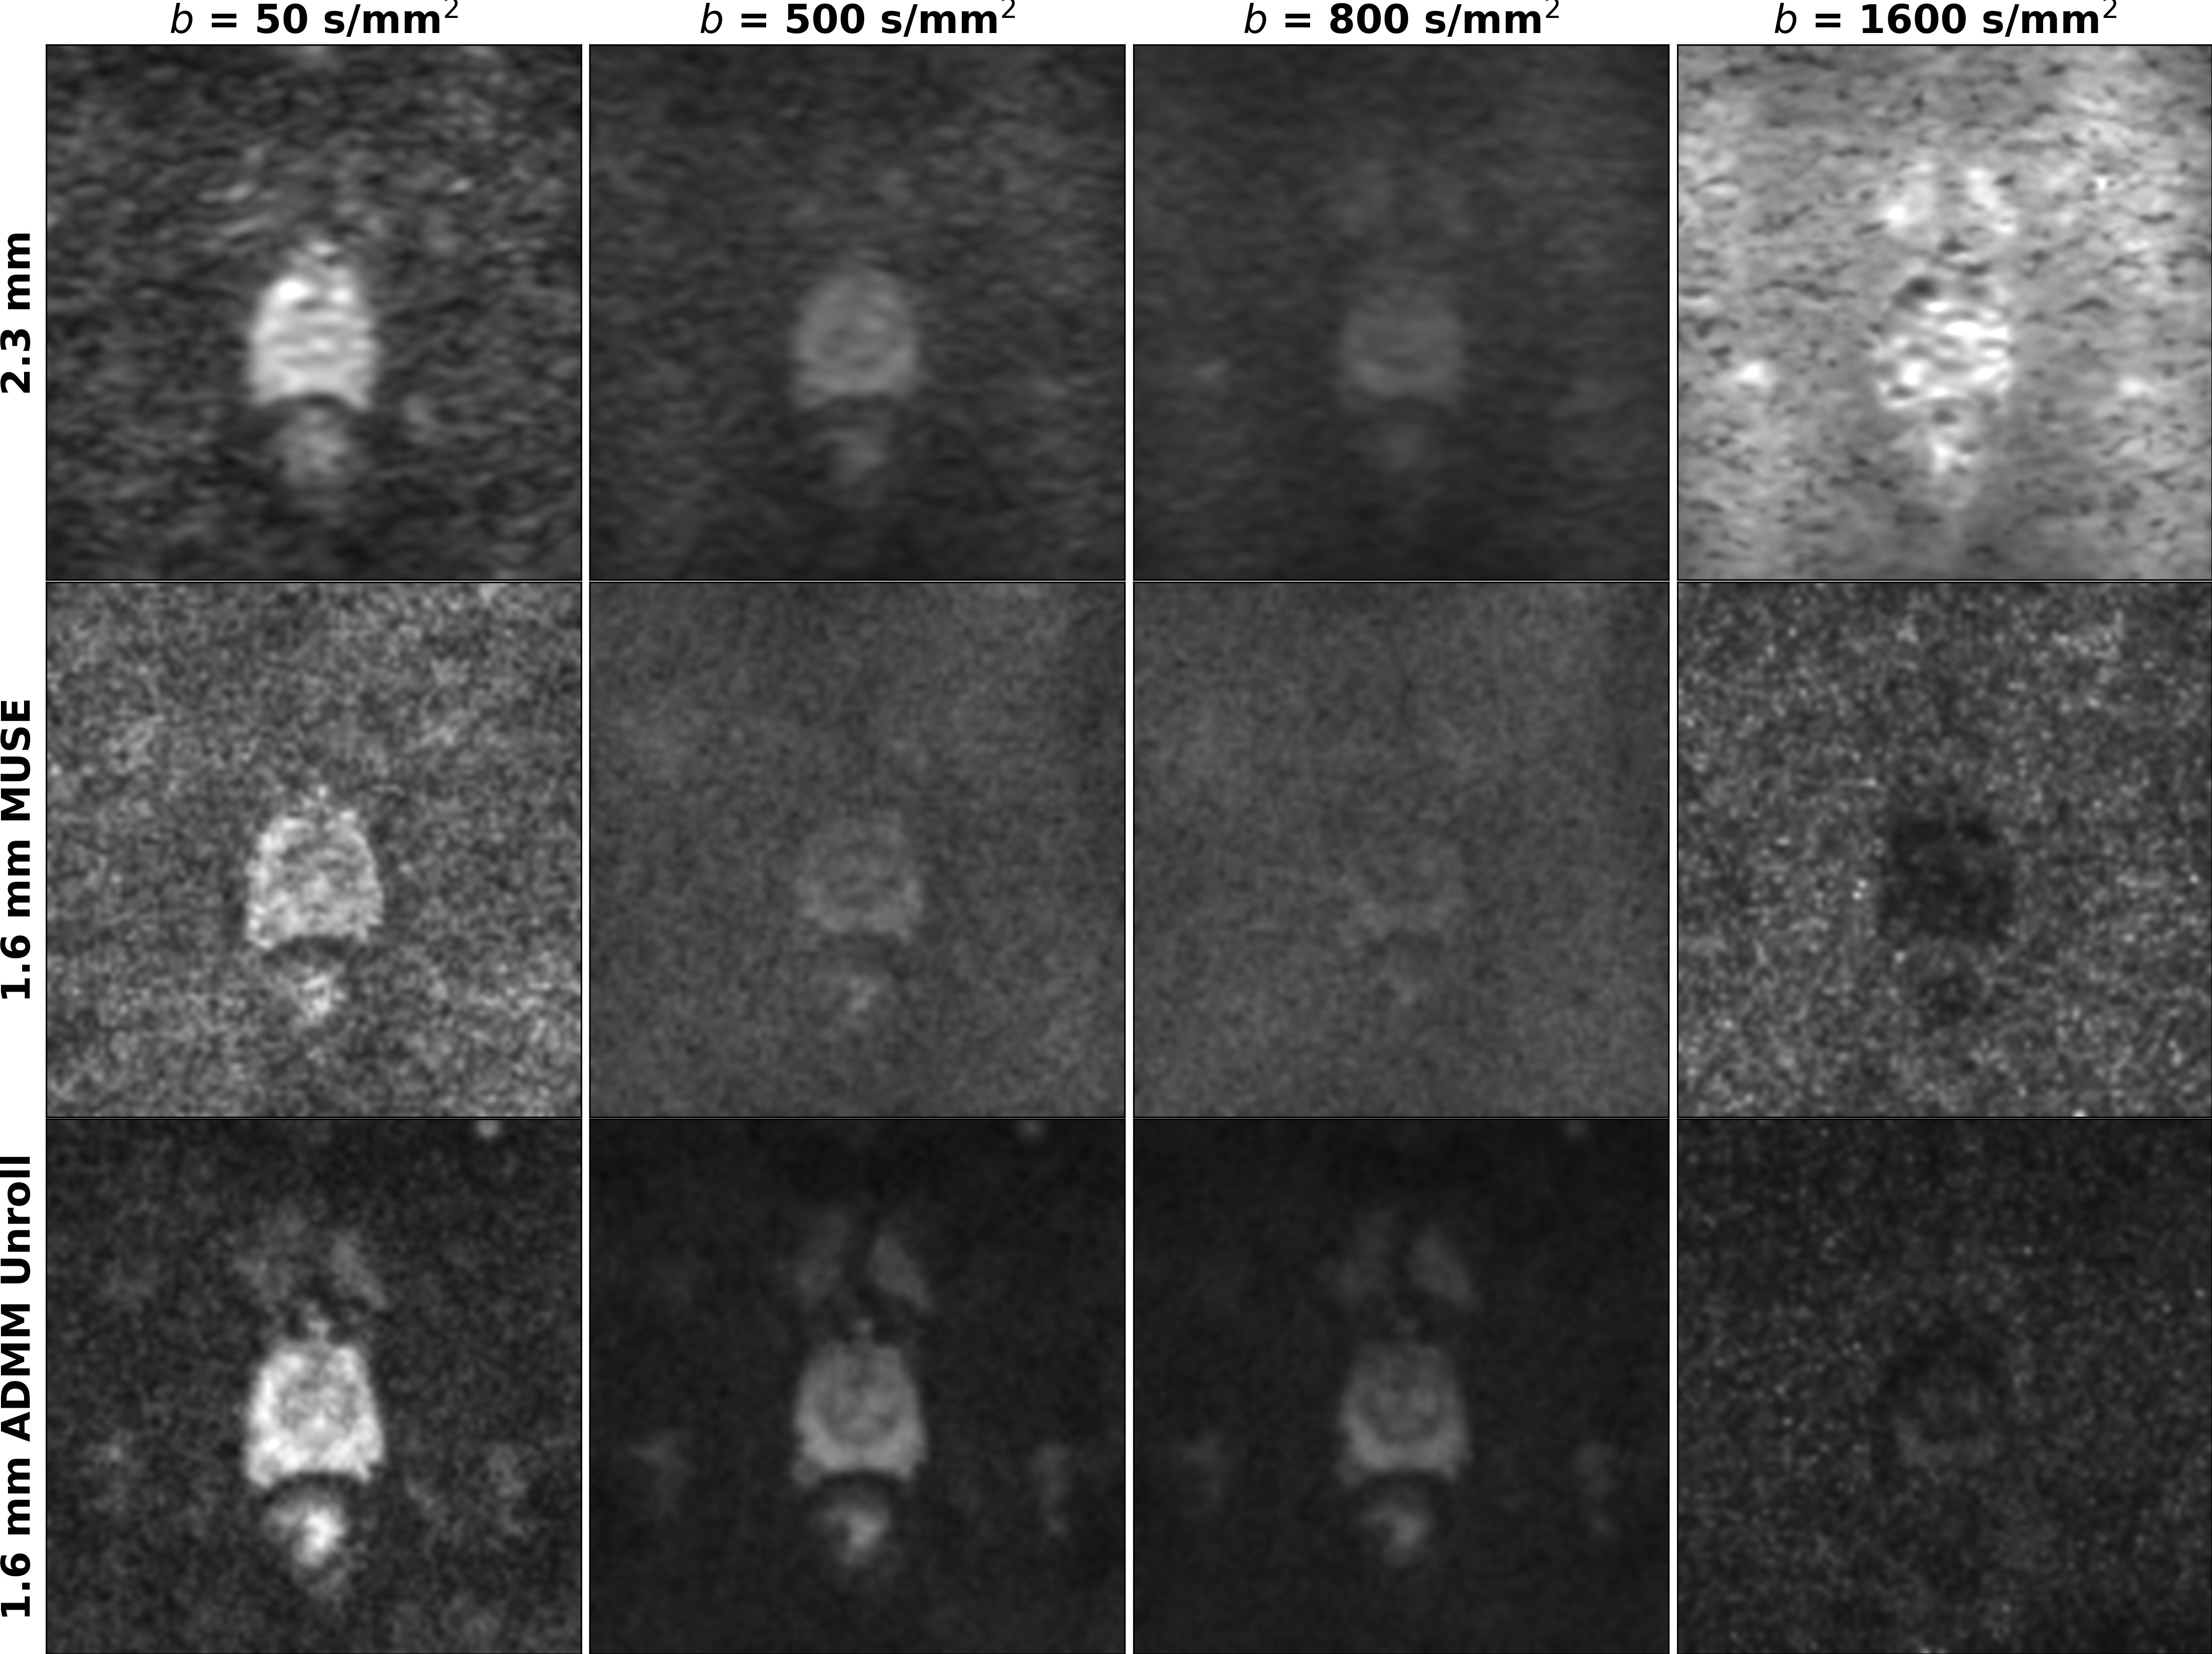
\includegraphics[width=\linewidth]{figures/2025-12-01_trace.png}
			\end{minipage}
			\hfill
			\begin{minipage}[t]{0.33\linewidth}
				\vspace{0pt}
				\captionof{figure}{Trace-weighted (TRACE) images from acquired $b$-values (\nth{1}-\nth{3} columns) 
					synthesized at $b=1600~\textnormal{s}/\textnormal{mm}^2$ (\nth{4} column).
					Compared to MUSE, ADMM unrolling substantially reduces noise in all TRACE images.
					Further, our calculated TRACE image 
					shows more reasonable contrast than that from the vendor, 
					which shows hyperintensity within the prostate.
					such hyerintensity is considered as an indicator of lesions.
					Since the volunteer reported no known prostate cancer prior to the experiment, 
					the hyperintensity from the vendor TRACE image is likely contaminated by noise.
				}
			\end{minipage}
			
			\vspace{5pt}

			\begin{minipage}[t]{0.60\linewidth}
				\vspace{0pt}
				\centering
				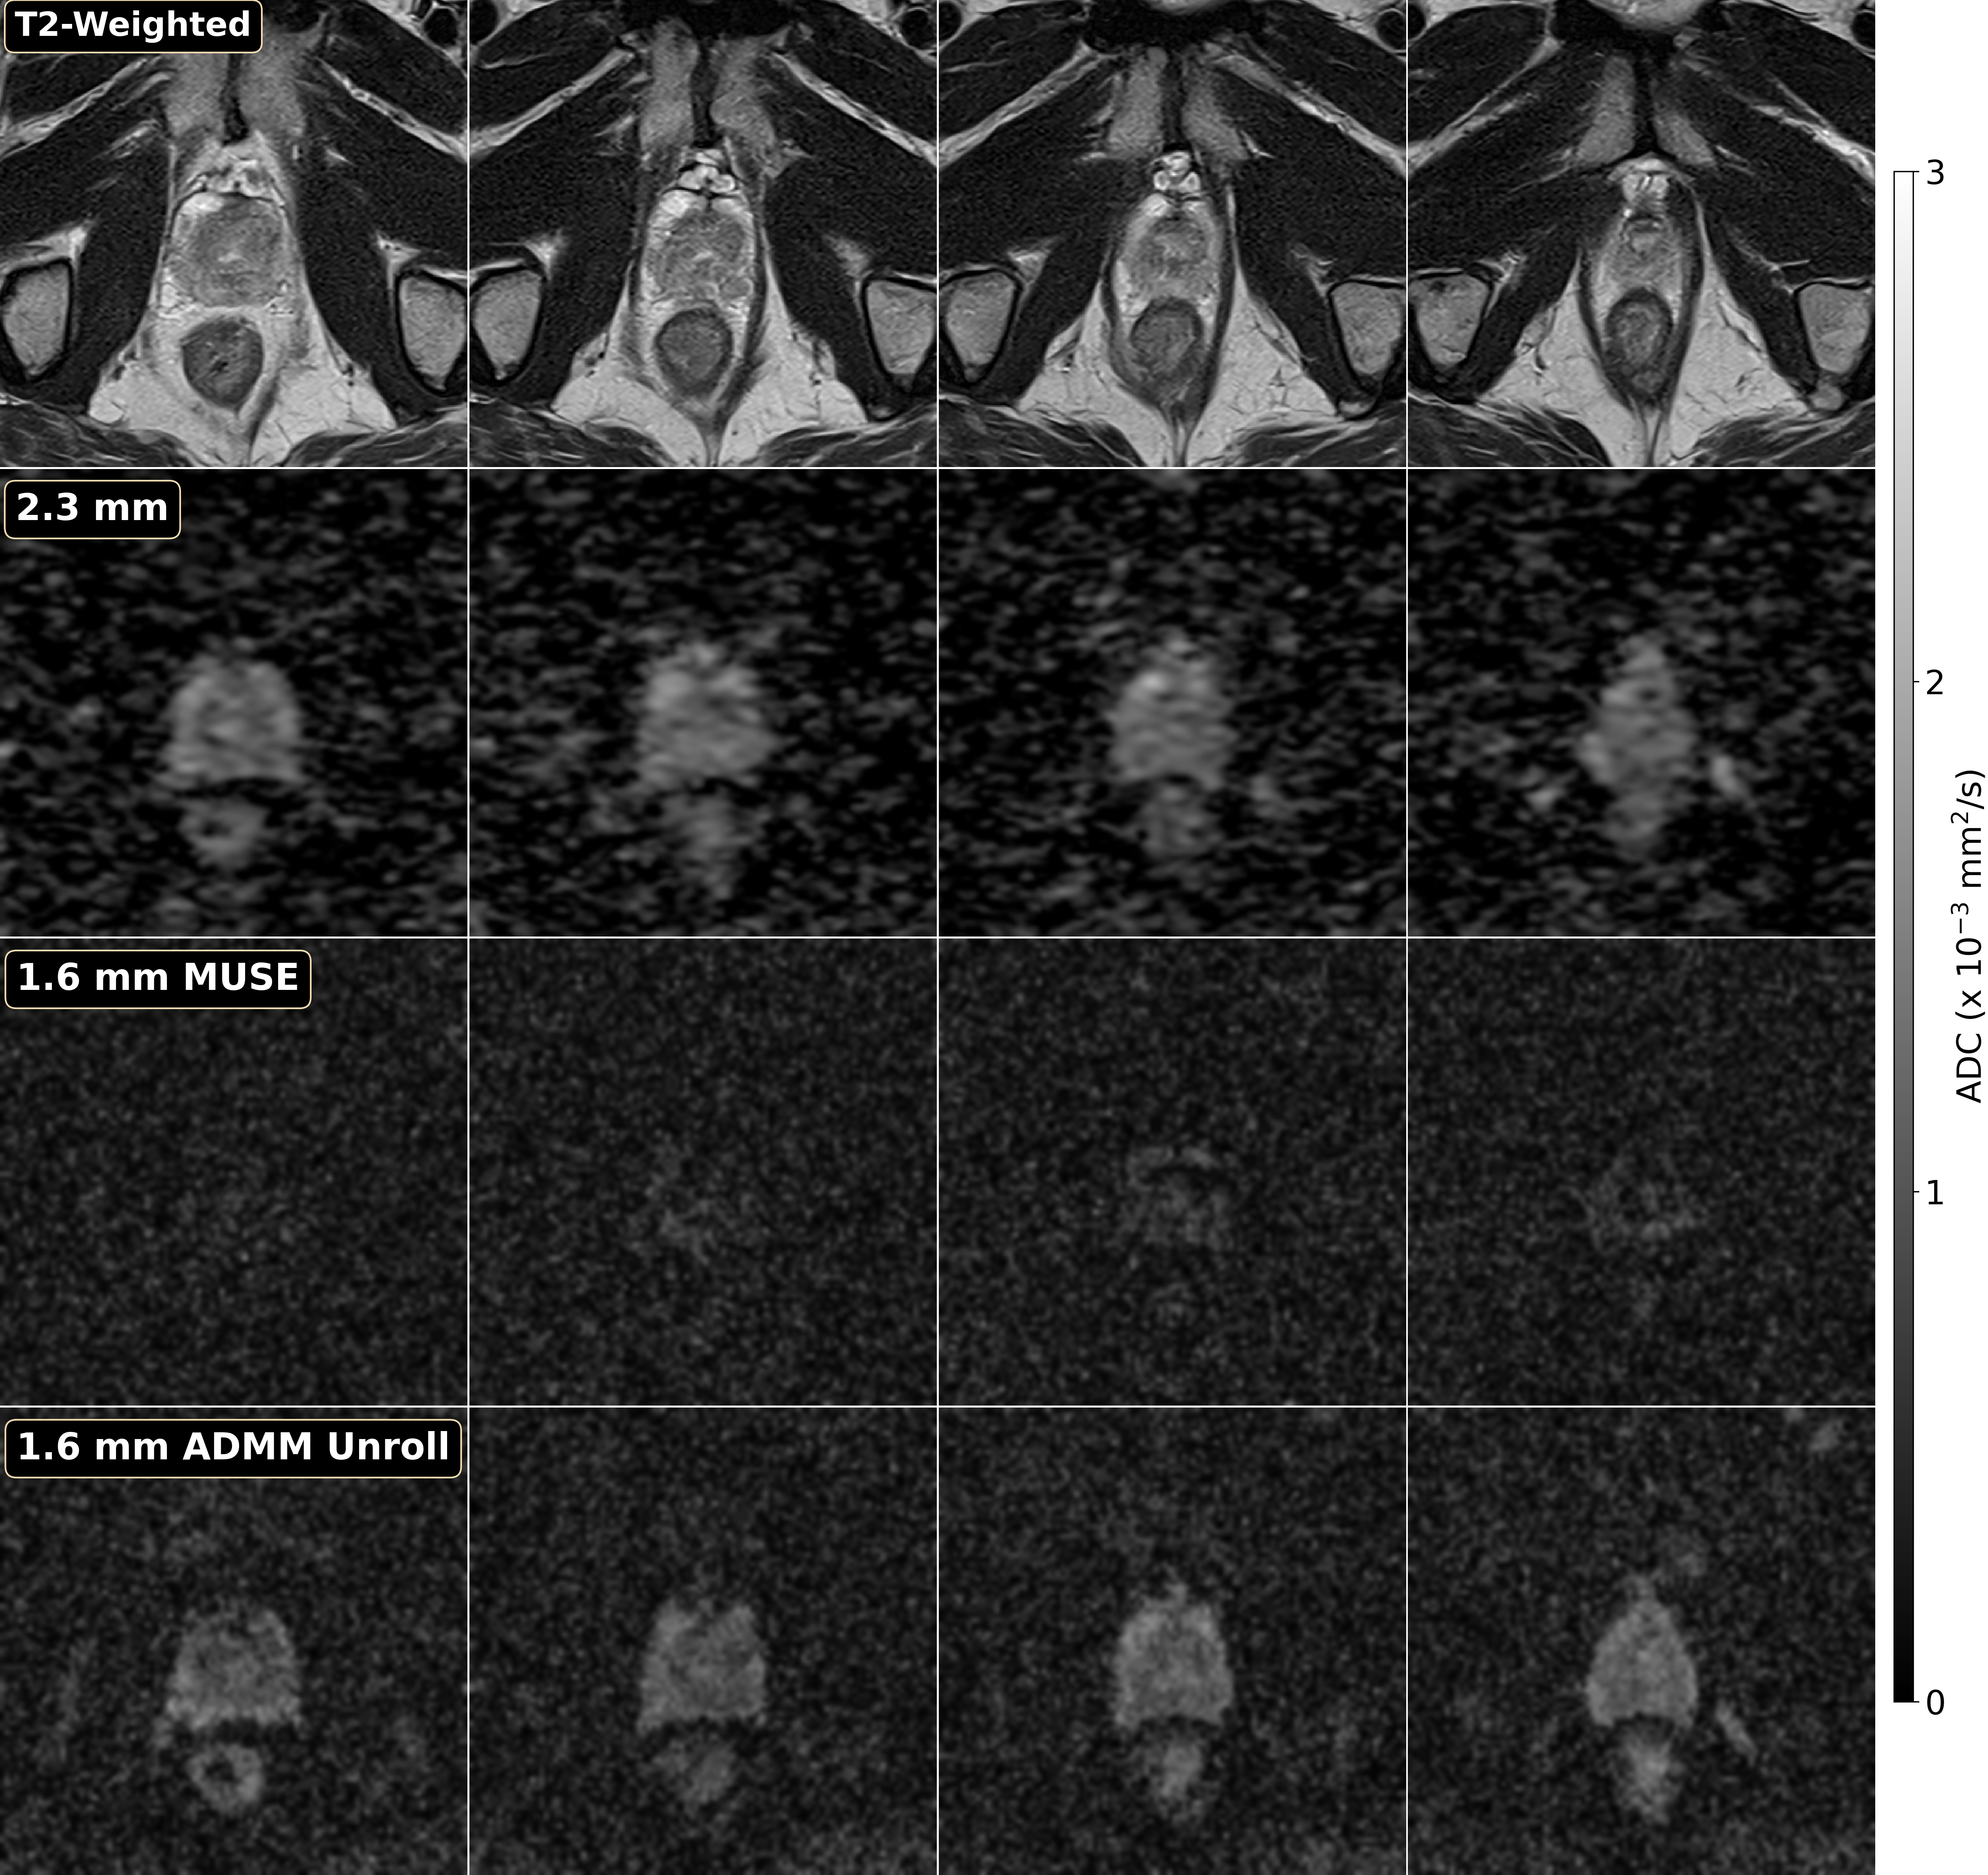
\includegraphics[width=\linewidth]{figures/2025-12-01_adc.png}
			\end{minipage}
			\hfill
			\begin{minipage}[t]{0.33\linewidth}
				\vspace{0pt}
				\captionof{figure}{
					(\nth{1} row) $T_2$-weighted images from four consecutive slices.
					(\nth{2} row) ADC maps acquired with Protocol \#1 and reconstructed by the vendor.
					(\nth{3} and \nth{4} rows) ADC maps acquired with Protocol \#2 and reconstructure by MUSE and ADMM unrolling, respectively.
					The vendor reconstructed ADC maps from Protocol \#1 suffers from blurry artifacts and 
					it is difficult to distinguish the peripheral from the central zone. 
					The use of 2-shot EPI in Protocol \#2 improves spatial resolution, but the reduced voxel size poses SNR penalty. 
					This is evident in MUSE (\nth{3} row), 
					from which the entire prostate region shows no visible signal. 
					Our proposed ADMM unrolling addresses the SNR challenge. All ADC maps shows comparable signal as the vendor reconstruction 
					and displays sharper delineation of the prostate anatomy in all slices.
				}
			\end{minipage}
		}

		\mtblock{4cm}{4. REFERENCE}{
			\begin{enumerate}[label={[\arabic*]},noitemsep]
				\item Weinreb JC, et al. PI-RADS prostate imaging - reporting and data systems: 2015, Version 2. \textit{Eur Urol} (2016).
				\item \textbf{Tan Z}, et al. JETS-NAViEPI. \textit{Imaging Neuroscience} (2024). \href{https://doi.org/10.1162/imag_a_00085}{10.1162/imag\_a\_00085}
				\item Monga V, et al. Algorithm Unrolling: Interpretable, Efficient Deep Learning for Signal and Image Processing. \textit{IEEE Trans Signal Process Mag} (2021). \href{https://ieeexplore.ieee.org/stamp/stamp.jsp?arnumber=9363511}{10.1109/MSP.2020.3016905}
				\item \textbf{Tan Z}, et al. High-resolution diffusion-weighted imaging with self-gated self-supervised unrolled reconstruction. \textit{Magn Reson Med} (2026). \href{https://doi.org/10.1002/mrm.70250}{10.1002/mrm.70250}
				\item Yaman B, et al. SSDU. \textit{Magn Reson Med} (2020). \href{https://doi.org/10.1002/mrm.28378}{10.1002/mrm.28378}
				\item He K, et al. Deep residual learning for image recognition. \textit{CVPR} (2016). \href{https://ieeexplore.ieee.org/stamp/stamp.jsp?arnumber=7780459}{10.1109/CVPR.2016.90}
				\item Chen NK, et al. MUSE. \textit{NeuroImage} (2013). \href{https://doi.org/10.1016/j.neuroimage.2013.01.038}{10.1016/j.neuroimage.2013.01.038}
			\end{enumerate}
		}

		{e-mail \texttt{welcome@overleaf.com}}
	\end{columns}

\end{document}